\documentclass[master]{outhesis}

\title{Master's Thesis}
\author{Bryan Hoke}
\degreename{Master of Science in Computer Science}
\school{University of Oklahoma}
\chair{Dr. Dean Hougen}

\usepackage{amsmath}
\usepackage{graphicx}
\usepackage{float}

\graphicspath{ {Figures/} }

\newcommand{\mutationrate}{0.1}
\newcommand{\crossoverrate}{0.8}
\newcommand{\populationsize}{40}
\newcommand{\learningrulesize}{35}

\begin{document}
\makefrontmatter

% Procedure
\chapter{Procedure}

%% Implementation Details
\section{Implementation Details}

%%% Genetic Coding of Learning Mechanisms
\subsection{Genetic Coding of Learning Mechanisms}

\begin{center}
	$a_j$ the activation of the input unit $j$
\end{center}

\begin{center}
	$o_i$ the activation of the output unit $i$
\end{center}

\begin{center}
	$t_i$ the training signal on output unit $i$
\end{center}

\begin{center}
	$w_{ij}$ the current value of the connection strength from input $j$ to output $i$
\end{center}

The genome encodes a function $F$ such that

\[
	\Delta w_{ij} = F(a_j, o_i, t_i, w_{ij})
\]

$F$ is a linear function of its four parameters and their six pairwise products. Thus $F$ is determined by specifying ten coefficients.

The genome encodes these ten coefficients, as well as an eleventh "scale" parameter.

\[
	\Delta w_{ij} = k_0(k_1w_{ij}+k_2a_j+k_3o_i+k_4t_i+k_5w_{ij}a_j+k_6w_{ij}o_i+k_7w_{ij}t_{i}+k_8a_jo_i+k_9a_jt_i+k_{10}o_it_i)
\]

The portion of the genome which encodes $\Delta w_{ij}$ consists of 35 bits. The first five bits encode the scale parameter $k_0$ such that it can represent the values $0$, $\pm 1/256$, $\pm 1/128$, ..., $\pm 32$, $\pm 64$, via exponential encoding. The first bit encodes the sign of $k_0$ (0: negative, 1: positive), and the next four bits encode the magnitude. If these four bits are interpreted as an integer $j$ between 0 and 15, we have

\[
	|k_0|=
	\begin{cases}
		0 & \text{if $j = 0$}\\
		2^{j-9} & \text{if $j = 1, ..., 15$}
	\end{cases}
\]

The other 30 bits encode the other ten coefficients in groups of three. The first bit of each group expresses the sign, and the other two bits express a magnitude of 0, 1, 2, or 4 via a similar exponential encoding. If we interpret these two bits as an integer $j$ between 0 and 3, then

\[
	|k_i|=
	\begin{cases}
		0 & \text{if $j = 0$}\\
		2^{j-1} & \text{if $j = 1, 2, 3$}
	\end{cases}
\]

%%% Genetic Coding of Initial Weights
\subsection{Genetic Coding of Initial Weights}

Network weights are evolved alongside learning rules. It would not be meaningful for each chromosome to represent a single set of weights to be used on all tasks, so instead each chromosome simultaneously represents a distinct set of weights for every task in the evolutionary run. The weights to be applied to each evolutionary task are encoded in distinct, consistent regions of each chromosome. 

\newcommand{\bitsperweight}{3}
\newcommand{\jlen}{2}
\newcommand{\jmin}{0}
\newcommand{\jmax}{3}
\newcommand{\exponentshift}{4}

Weights are encoded using 3 bits each. The first bit is the sign of the weight. If we interpret these two bits as an integer $j$ between 0 and 3, then

\[
	|k_i|=
	\begin{cases}
		0 & \text{if $j = 0$}\\
		2^{j-4} & \text{if $j = 1, 2, 3$}
	\end{cases}
\]

For each task the number of weights encoded is equal to the number of inputs in that task plus one bias weight.

There are two conditions of evaluation: the "nurturing" case and the "non-nurturing" case. During evaluation, each network is first trained for 10 epochs using its learning rule. Following this, the network is evaluated on the same tasks. In the "nurturing" case the individual's fitness is simply the result of the evaluation, whereas in the "non-nurturing" case the individual's fitness is the average of evaluation during all training epochs and the final evaluation.

%%% Evaluation of Fitness
\subsection{Evaluation of Fitness}

Fitness evaluation for the nurturing case:

(1) Create a network with the appropriate number of input units for the task and a single output unit.

(2) Initialize the connection strengths of the network using the values encoded in the chromosome

(3) For 10 epochs, cycle through the training exemplars for the task, where for each exemplar we:

(3a) Propagate input values through the system, yielding output values; then

(3b) Adjust the weights of the system according to the formula specified by the learning procedure, on the basis of inputs, output, training signal, and current weights.

(4) At the end of this process, fitness on the task is measured by testing the network on all training exemplars, and dividing the total error by the number of exemplars, subtracting from 1, and multiplying by 100. This yields a fitness "percentage" between 0 and 100.

Fitness evaluation for the non-nurturing case:

(1) Create a network with the appropriate number of input units for the task and a single output unit.

(2) Initialize the connection strengths of the network using the values encoded in the chromosome

(3) For 10 epochs, cycle through the training exemplars for the task, where for each exemplar we:

(3a) Test the network on the exemplar and measure the error in the network output; then

(3b) Propagate input values through the system, yielding output values, then adjust the weights of the system according to the formula specified by the learning procedure, on the basis of inputs, output, training signal, and current weights.

(4) At the end of this process, test the network on all training exemplars and divide the total error of this test and all tests from step 3a by the total number of tests that occurred, subtracting from 1, and multiplying by 100. This yields a fitness "percentage" between 0 and 100.

Fitness of the chromosome is obtained by evaluating its performance on each of the (typically 20) tasks, and taking the mean fitness over all tasks. In this way every chromosome is assigned a fitness between 0 and 100\%.

%%% Parameters of the Genetic Algorithm
\subsection{Parameters of the Genetic Algorithm}

% TODO: Describe GA used
% TODO: Describe "segment-wise" crossover used

Population size: 40
Crossover rate: 0.8
Mutation rate: 0.01
Elitism factor: 1
Number of generations: 4000

%%% Post-Evolutionary Evaluation
\subsection{Post-Evolutionary Evaluation}

Before each evolutionary run, 10 tasks are selected from the task pool and designated as "test tasks". After each evolutionary run, the chromosome with the highest fitness score in the history of the populations in that run is identified. From this chromosome, the learning rule bits are isolated and evaluated on the test tasks (using both the nurturing and non-nurturing conditions) and the weight-encoding bits are isolated and evaluated on the evolutionary tasks.

% Results
\chapter{Results}

%% Results of initial evolutionary runs
\section{Results of initial evolutionary runs}

%% Fitness test
\section{Fitness test}

\begin{figure}[H]
	\centering
	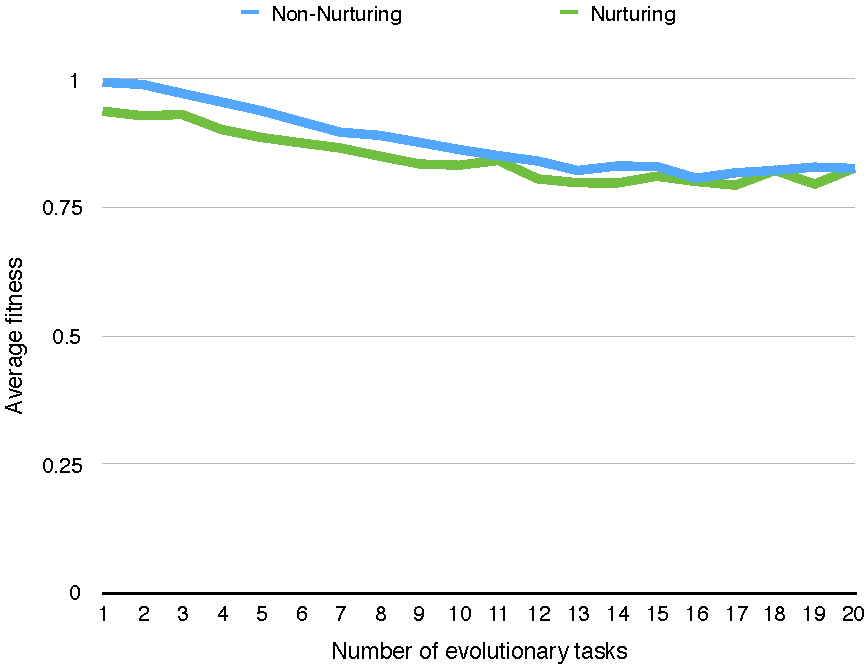
\includegraphics{NonNurturingFitnessTestPlot.pdf}
	\caption{Non-nurturing fitness test on evolutionary tasks.}
\end{figure}

\begin{figure}[H]
	\centering
	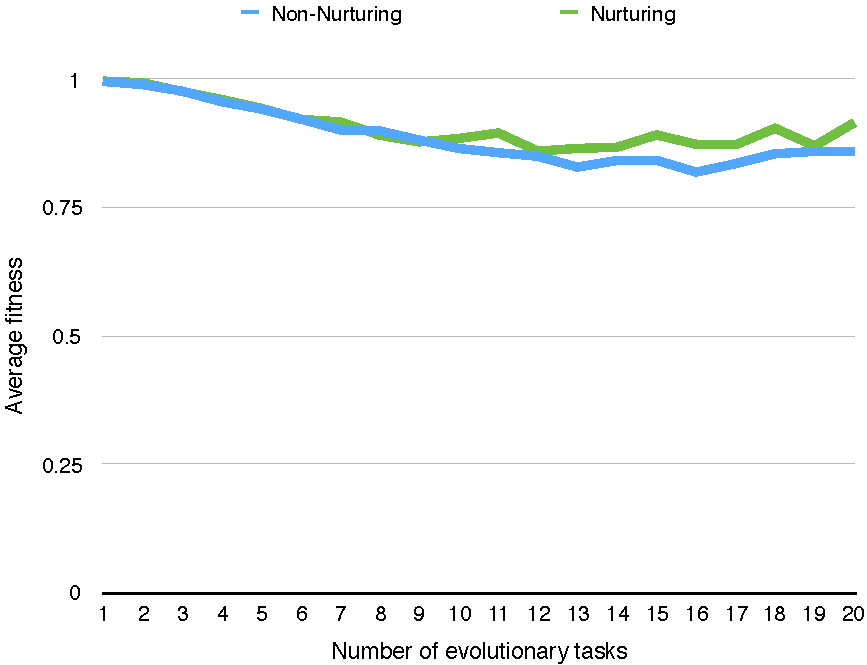
\includegraphics{NurturingFitnessTestPlot.pdf}
	\caption{Nurturing fitness test on evolutionary tasks.}
\end{figure}

%% Network test
\section{Network test}

\begin{figure}[H]
	\centering
	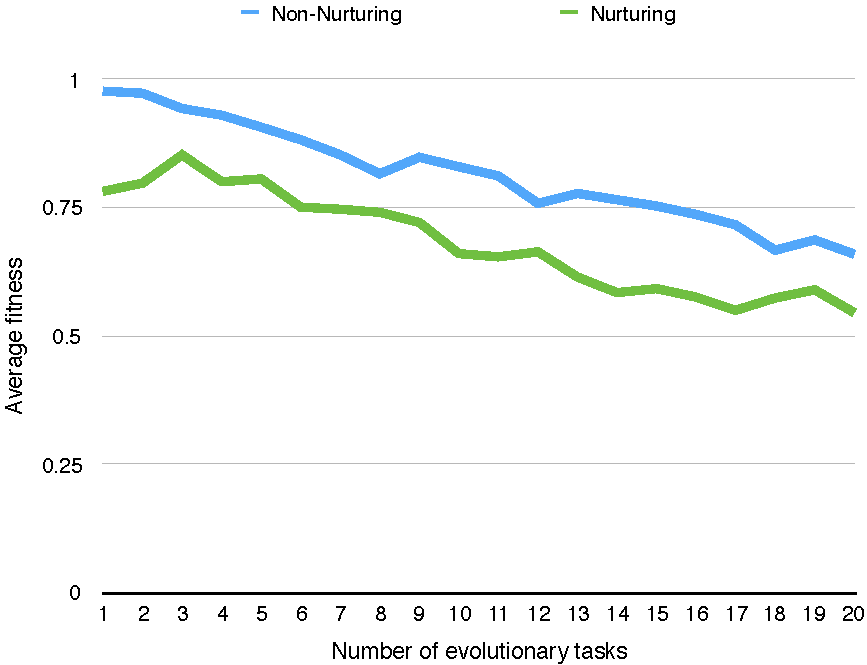
\includegraphics{NetworkTestPlot.pdf}
	\caption{Network test on evolutionary tasks.}
\end{figure}

%% Generalization test
\section{Generalization test}

\begin{figure}[H]
	\centering
	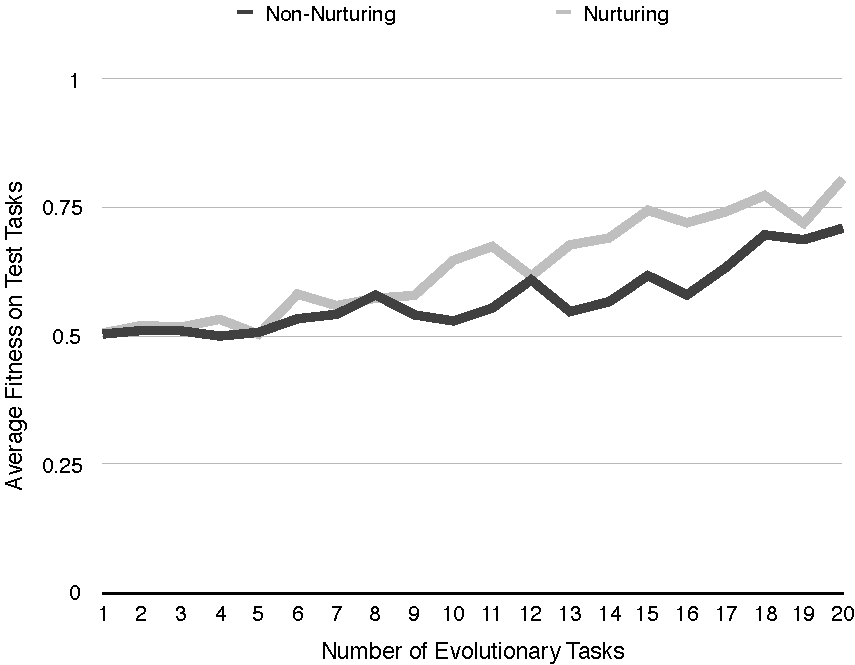
\includegraphics{NonNurturingGeneralizationTestPlot.pdf}
	\caption{Non-nurturing generalization test on test tasks.}
\end{figure}

\begin{figure}[H]
	\centering
	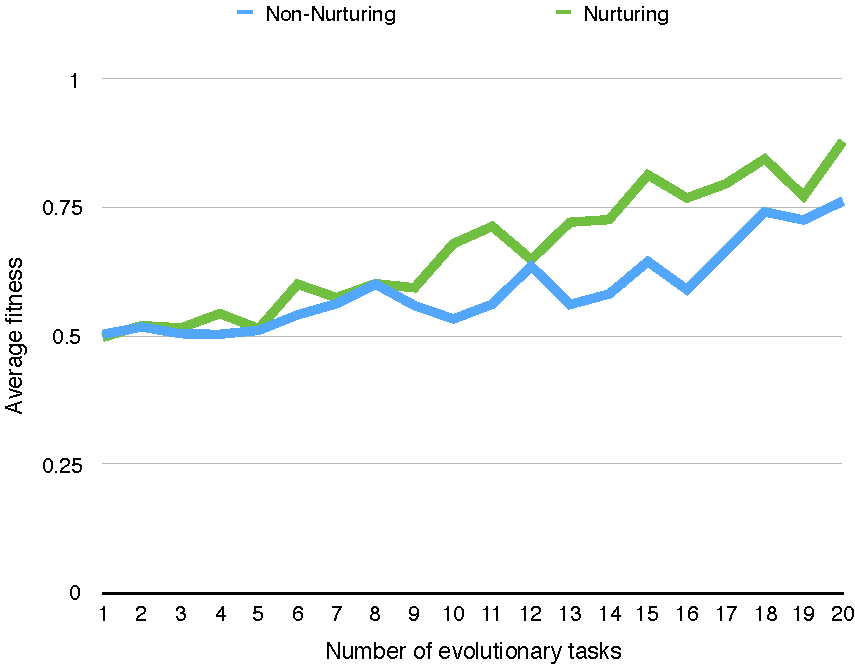
\includegraphics{NurturingGeneralizationTestPlot.pdf}
	\caption{Nurturing generalization test on test tasks.}
\end{figure}

%% Learning test
\section{Learning test}

\begin{figure}[H]
	\centering
	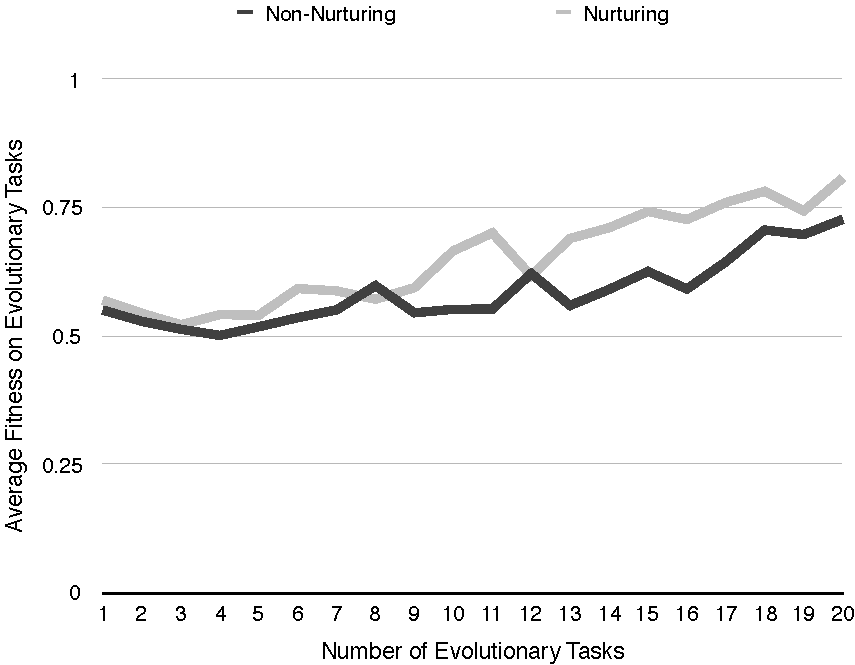
\includegraphics{NonNurturingLearningTestPlot.pdf}
	\caption{Non-nurturing learning test on test tasks.}
\end{figure}

\begin{figure}[H]
	\centering
	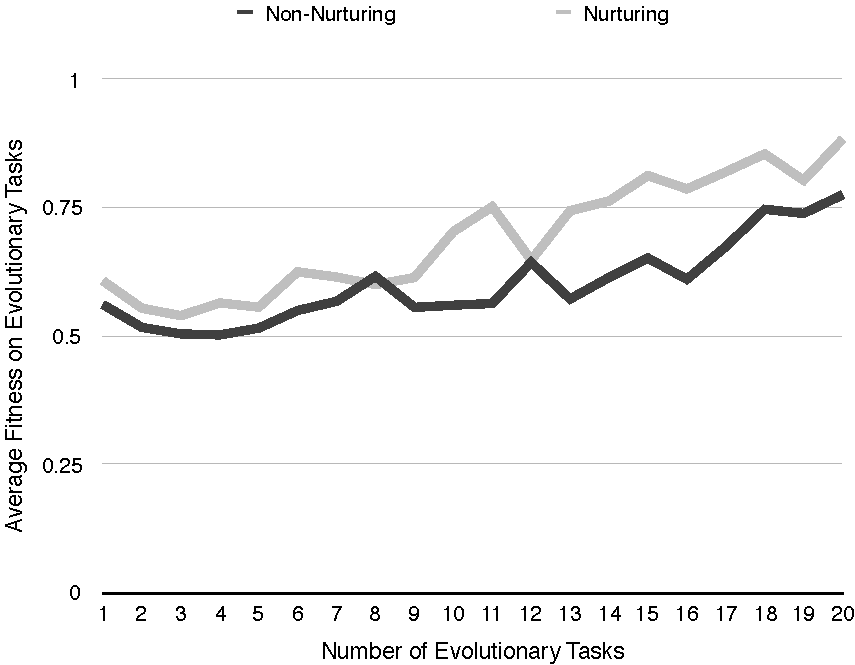
\includegraphics{NurturingLearningTestPlot.pdf}
	\caption{Nurturing learning test on test tasks.}
\end{figure}

\makebackmatter
\end{document}